\documentclass[aspectratio=169,unicode,compress,14pt]{beamer}
\usepackage{luatexja-preset,amsmath,ulem,tikz,here,color,hyperref}
\def\aatitle{Opeth, Lua VM Bytecode Optimizer}
\usetikzlibrary{shapes,snakes,arrows.meta,positioning,calc}
\def\nodecolor{blue!20}%
\input{../template/beamertemp.tex}
\input{../template/mylisting.tex}
\setmonofont{Meslo LG L}
\setsansfont{Source Han Sans JP}
\setsansjfont{Source Han Sans JP}
\setromanfont{Takao Ex Mincho}
\setmainfont{Source Han Sans JP}
\setmainjfont{Source Han Sans JP}
\setbeamersize{text margin left=1\zw}
\setbeamersize{text margin right=1\zw}
\newfontfamily{\theking}{theKing26Queen}
\newcommand{\Opeth}{\textcolor{black}{{\huge{}Opeth}{\footnotesize{},\\Lua VM Bytecode Optimizer}}}
\title{\Opeth}
\keywords{Lua VM, Register-based VM, optimization}
\author{\footnotesize{}Nymphium}
\date{\footnotesize{}February 12, 2017 at tsukuba.lua}
\makeatletter
\hypersetup{
	pdftex,
	pdftitle=\aatitle,
	pdfsubject=\aatitle,
	pdfauthor={びしょ〜じょ},
	pdfkeywords={Optimization, Register-based Virtual Machine, Lua},
	urlcolor=blue,
	colorlinks=false,
	% pdfborderstyle={/S/U/W .5}
}
\makeatother
\begin{document}
\bgroup
\theking
\maketitle
\egroup
\title{\aatitle}
\skipnexttoc
\section{Today's Topic}
\begin{frame}
  \frametitlesec

  By the way, do you...

  \large
  \begin{itemize}[<+->]
    \pause
    \item[\emoji{woman-raising-hand}] Use Go Compiler?

    \item[\large \emoji{woman-raising-hand}] {\large Use Optimization?}

    \item[] Then,

      \onslide<+->{
        \huge\vspace*{0.5\zh}\emoji{woman-raising-hand}\vspace*{-2\zh}
        \begin{center}
          \color{red}
          Use

          Profile-Guilded

          Optimization?
        \end{center}
      }
  \end{itemize}
\end{frame}

\begin{frame}
  \frametitlesec
  \Large
  \semibf

  \centering

  Learn about\pause

  \vspace*{15pt}
  {\scalefont{1.8}\color{red}\textbfslant{Profile-Guilded Optimization}}\pause
  \vspace*{6pt}

  and
  \vspace*{10pt}

  around \textcolor{blue}{\scalefont{1.5}its optimizations}

\end{frame}

\section{Opeth}
\begin{frame}
	\frametitlesec
	Q. Do you know a metal band, {\theking{}Opeth} ?

	\pause\vskip3\zw

	\begin{figure}
		\centering
		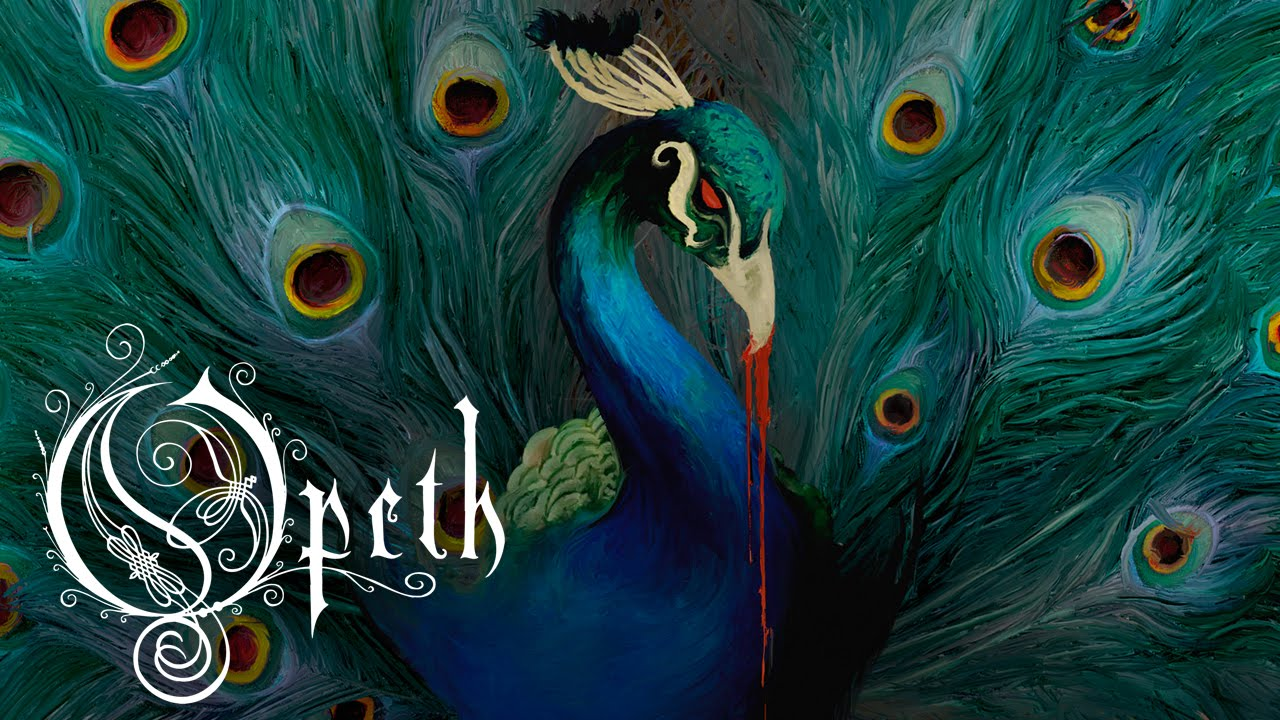
\includegraphics[height=.4\textheight]{img/opeth_newalbum.png}
		\caption{Opeth、新譜出すってよ}
	\end{figure}
\end{frame}
\section{Today's Topic}
\begin{frame}
  \frametitlesec

  By the way, do you...

  \large
  \begin{itemize}[<+->]
    \pause
    \item[\emoji{woman-raising-hand}] Use Go Compiler?

    \item[\large \emoji{woman-raising-hand}] {\large Use Optimization?}

    \item[] Then,

      \onslide<+->{
        \huge\vspace*{0.5\zh}\emoji{woman-raising-hand}\vspace*{-2\zh}
        \begin{center}
          \color{red}
          Use

          Profile-Guilded

          Optimization?
        \end{center}
      }
  \end{itemize}
\end{frame}

\begin{frame}
  \frametitlesec
  \Large
  \semibf

  \centering

  Learn about\pause

  \vspace*{15pt}
  {\scalefont{1.8}\color{red}\textbfslant{Profile-Guilded Optimization}}\pause
  \vspace*{6pt}

  and
  \vspace*{10pt}

  around \textcolor{blue}{\scalefont{1.5}its optimizations}

\end{frame}


\section{implementation}

\section{tools}

\section{Conclusion}
\begin{frame}
\frametitlesec
\begin{itemize}
	\item 最適化器の実装
		\begin{itemize}
			\item 一部高速化に成功
			\item バイトコードの縮小化もぼちぼち
		\end{itemize}
	\item しんどかった
		\begin{itemize}
			\item ドキュメントは書こう
		\end{itemize}
	\item 課題
		\begin{itemize}
			\item 他の最適化も取り入れたい(for展開とか)
			\item 最適化器の最適化!
				\begin{itemize}
					\item アルゴリズムが適当すぎ
			\end{itemize}
		\end{itemize}
\end{itemize}
\end{frame}

\end{document}
